\documentclass[11pt, a4paper]{article}

% Fonts and Encoding
\usepackage[utf8]{inputenc}
\usepackage[T1]{fontenc}

% Math and Symbols
\usepackage{amsmath, amssymb, amsthm, amsfonts, mathrsfs, mathtools}

% Layout and Geometry
\usepackage{geometry}
\geometry{a4paper, margin=1in}

% Formatting and Graphics
\usepackage{graphicx, xcolor, enumitem, booktabs, array, tabularx}

% TikZ for Illustrations
\usepackage{tikz}
\usetikzlibrary{arrows.meta, positioning, shapes.geometric, calc, backgrounds, matrix}

% Clickable Links and TOC
\usepackage{hyperref}
\hypersetup{
    colorlinks=true,
    linkcolor=blue,
    filecolor=magenta,      
    urlcolor=cyan,
    pdftitle={Advanced Mathematics Topic: Independent Random Variables},
}

% Theorem Environments
\newtheorem{theorem}{Theorem}[section]
\newtheorem{lemma}[theorem]{Lemma}
\newtheorem{proposition}[theorem]{Proposition}
\newtheorem{corollary}[theorem]{Corollary}
\theoremstyle{definition}
\newtheorem{definition}{Definition}[section]
\newtheorem{axiom}{Axiom}[section]
\newtheorem{example}{Example}[section]
\theoremstyle{remark}
\newtheorem{remark}{Remark}[section]

% Custom Commands (Enforced standard notation)
\newcommand{\R}{\mathbb{R}}
\newcommand{\N}{\mathbb{N}}
\newcommand{\Z}{\mathbb{Z}}
\newcommand{\Q}{\mathbb{Q}}
\newcommand{\E}{\mathbb{E}}
\newcommand{\Prob}{\mathbb{P}}
\newcommand{\F}{\mathcal{F}}
\newcommand{\indep}{\perp\!\!\!\perp}

\title{\textbf{Advanced Multivariate Probability: \\ Independent Random Variables}}
\author{Tashfeen Omran}
\date{\today}

\begin{document}

\maketitle
\tableofcontents
\newpage

\section{Part 1: Comprehensive Introduction, Context, and Prerequisites}

\subsection{Core Concepts \& Axioms}
In the rigorous study of probability theory, built upon the axiomatic foundation laid by Andrey Kolmogorov in 1933, a probability space is defined as a measure space $(\Omega, \F, \Prob)$. A random variable $Y$ is a measurable function mapping the sample space $\Omega$ to the real numbers $\R$. When dealing with multiple random variables, we are concerned with their joint behavior, governed by a joint probability measure.

The concept of \textbf{Independence} is arguably the most crucial structural assumption in probability theory. Two random variables $Y_1$ and $Y_2$ are independent if the realization of one provides absolutely no information about the realization of the other. Formally, this means the joint cumulative distribution function (CDF) factors into the product of their marginal CDFs.

\begin{definition}[Independence of Random Variables]
Let $Y_1$ and $Y_2$ be random variables with joint CDF $F(y_1, y_2)$ and marginal CDFs $F_1(y_1)$ and $F_2(y_2)$. $Y_1$ and $Y_2$ are said to be \textbf{independent} (denoted $Y_1 \indep Y_2$) if and only if:
\[ F(y_1, y_2) = F_1(y_1)F_2(y_2) \quad \text{for all } (y_1, y_2) \in \R^2 \]
\end{definition}

\subsection{Intuition and Set-Theoretic Foundations}
From a set-theoretic perspective, events $A \in \F$ and $B \in \F$ are independent if $\Prob(A \cap B) = \Prob(A)\Prob(B)$. For random variables, we consider the pre-images of Borel sets. $Y_1$ and $Y_2$ are independent if the $\sigma$-algebras generated by them, $\sigma(Y_1)$ and $\sigma(Y_2)$, are independent. This means that for any Borel sets $B_1, B_2 \in \mathcal{B}(\R)$, the events $\{Y_1 \in B_1\}$ and $\{Y_2 \in B_2\}$ are independent. 

Visually, independence implies that the joint density (or mass) function is a "Cartesian product" of the marginals. If the support of the joint distribution (the region where the density is strictly positive) cannot be expressed as a Cartesian product of intervals (i.e., it is not a rectangle aligned with the axes), the variables \textit{cannot} be independent.

\subsection{Historical Context and Motivation}
Before the 1930s, probability was largely a collection of heuristic rules applied to gambling and physical sciences. The foundational crisis in mathematics at the turn of the 20th century demanded rigorous formalization. Kolmogorov utilized Lebesgue's measure theory to formalize probability. Independence, previously a vague notion of "unrelatedness," was rigorously defined as the factorization of product measures. This allowed mathematicians to prove powerful asymptotic results like the Strong Law of Large Numbers and the Central Limit Theorem, which strictly require sequences of independent random variables.

\subsection{Key Theorems and Lemmas}

\begin{theorem}[Density Factorization]
If $Y_1$ and $Y_2$ are jointly continuous (or discrete) with joint density (or mass) function $f(y_1, y_2)$ and marginals $f_1(y_1), f_2(y_2)$, they are independent if and only if:
\[ f(y_1, y_2) = f_1(y_1)f_2(y_2) \quad \text{for all } (y_1, y_2) \in \R^2 \]
\end{theorem}

\begin{theorem}[Support and Factorization (Theorem 5.5)]
Let $Y_1$ and $Y_2$ have a joint density $f(y_1, y_2)$ that is positive if and only if $a \le y_1 \le b$ and $c \le y_2 \le d$ (where $a,b,c,d$ are constants). Then $Y_1 \indep Y_2$ if and only if there exist non-negative functions $g(y_1)$ and $h(y_2)$ such that:
\[ f(y_1, y_2) = g(y_1)h(y_2) \]
\end{theorem}

\subsection{Prerequisites}
To master this section, one must possess:
\begin{itemize}
    \item \textbf{Multivariable Calculus:} Proficiency in double integration over non-rectangular regions.
    \item \textbf{Measure Theory Basics:} Understanding of support, marginalization (integrating out variables), and product spaces.
    \item \textbf{Logic:} Ability to prove statements using direct proof and proof by counterexample (especially for showing dependence).
\end{itemize}

\newpage
\section{Part 2: Detailed Homework Solutions}

\subsection{Theoretical Proofs (5.43 - 5.44)}

\textbf{Exercise 5.43:} Let $Y_1, Y_2$ have joint density $f(y_1, y_2)$ and marginals $f_1(y_1), f_2(y_2)$. Show $Y_1 \indep Y_2 \iff f(y_1|y_2) = f_1(y_1)$ for all $y_1$ and all $y_2$ such that $f_2(y_2) > 0$.
\begin{proof}
\textit{Forward Direction ($\implies$):} Assume $Y_1 \indep Y_2$. By definition, $f(y_1, y_2) = f_1(y_1)f_2(y_2)$. The conditional density is defined as:
\[ f(y_1|y_2) = \frac{f(y_1, y_2)}{f_2(y_2)} \]
Substituting the independence condition:
\[ f(y_1|y_2) = \frac{f_1(y_1)f_2(y_2)}{f_2(y_2)} = f_1(y_1) \]
\textit{Reverse Direction ($\impliedby$):} Assume $f(y_1|y_2) = f_1(y_1)$ for all $y_2$ where $f_2(y_2) > 0$. By the definition of conditional probability:
\[ f(y_1, y_2) = f(y_1|y_2)f_2(y_2) \]
Substituting the assumption yields $f(y_1, y_2) = f_1(y_1)f_2(y_2)$, which is the definition of independence. $\blacksquare$
\end{proof}

\textbf{Exercise 5.44:} Prove that the results in Exercise 5.43 also hold for discrete random variables.
\begin{proof}
The proof is identical to 5.43, replacing the probability density functions $f$ with probability mass functions $p$.
Assume $Y_1 \indep Y_2$. Then $p(y_1, y_2) = p_1(y_1)p_2(y_2)$.
\[ p(y_1|y_2) = \frac{p(y_1, y_2)}{p_2(y_2)} = \frac{p_1(y_1)p_2(y_2)}{p_2(y_2)} = p_1(y_1) \]
Conversely, if $p(y_1|y_2) = p_1(y_1)$, then $p(y_1, y_2) = p(y_1|y_2)p_2(y_2) = p_1(y_1)p_2(y_2)$, establishing independence. $\blacksquare$
\end{proof}

\subsection{Discrete Joint Distributions (5.45 - 5.48)}

\textbf{Exercise 5.45:} Are $Y_1$ and $Y_2$ independent based on the provided table?
\begin{proof}
We are given $p_1(y_1)$ is Binomial with $n=2, p=1/3$. Thus, $p_1(0) = \binom{2}{0}(1/3)^0(2/3)^2 = 4/9$.
From the table, the marginal probability $p_2(0)$ is the sum of the first row:
\[ p_2(0) = 1/9 + 2/9 + 1/9 = 4/9 \]
For independence to hold, we must have $p(y_1, y_2) = p_1(y_1)p_2(y_2)$ for all pairs. Let us test $(0,0)$:
\[ p(0,0) = 1/9 \]
\[ p_1(0)p_2(0) = (4/9) \times (4/9) = 16/81 \]
Since $1/9 \neq 16/81$, the condition fails. Therefore, $Y_1$ and $Y_2$ are \textbf{dependent}. $\blacksquare$
\end{proof}

\textbf{Exercise 5.46:} 3 coin tosses. $Y_1$ = total heads, $Y_2$ = winnings on side bet. Are they independent?
\begin{proof}
The winnings $Y_2$ are a deterministic function of the number of heads $Y_1$. If we know $Y_1$, we know $Y_2$ with probability 1. For example, let $A$ be the event $\{Y_1 = 0\}$ and $B$ be the event $\{Y_2 = w_0\}$ (where $w_0$ is the payout for 0 heads).
\[ \Prob(Y_2 = w_0 \mid Y_1 = 0) = 1 \neq \Prob(Y_2 = w_0) \]
Because the conditional probability does not equal the marginal probability, they are \textbf{dependent}. $\blacksquare$
\end{proof}

\textbf{Exercise 5.47:} $p(y_1, y_2) = \binom{4}{y_1}\binom{3}{y_2}\binom{2}{3-y_1-y_2} / \binom{9}{3}$. Are $Y_1, Y_2$ independent?
\begin{proof}
Observe the support constraints: $0 \le y_1 \le 3$, $0 \le y_2 \le 3$, and $1 \le y_1 + y_2 \le 3$.
Because the upper bound of $y_2$ depends on the value of $y_1$ (specifically, $y_2 \le 3 - y_1$), the support is not a Cartesian product of independent intervals. 
For example, $p(3, 3) = 0$, but $p_1(3) > 0$ and $p_2(3) > 0$. Thus $p(3,3) \neq p_1(3)p_2(3)$. They are \textbf{dependent}. $\blacksquare$
\end{proof}

\textbf{Exercise 5.48:} Are $Y_1$ (child survived) and $Y_2$ (belt used) independent?
\begin{proof}
From the provided table, we extract the joint and marginal probabilities for the cell $(0,0)$:
\[ p(0,0) = 0.38 \]
\[ p_1(0) = 0.55 \quad \text{and} \quad p_2(0) = 0.76 \]
We check the factorization condition:
\[ p_1(0)p_2(0) = 0.55 \times 0.76 = 0.418 \]
Since $0.38 \neq 0.418$, the variables are \textbf{dependent}. $\blacksquare$
\end{proof}

\subsection{Continuous Joint Distributions: Support Checks (5.49 - 5.61)}

\textbf{Exercise 5.49:} $f(y_1, y_2) = 3y_1$ for $0 \le y_2 \le y_1 \le 1$. Show dependence.
\begin{proof}
The support is defined by $0 \le y_2 \le y_1 \le 1$. The boundaries of $y_2$ depend on the realization of $y_1$. Because the support region is a triangle and not a rectangle (Cartesian product of intervals), Theorem 5.5 cannot be satisfied. Thus, $Y_1$ and $Y_2$ are \textbf{dependent}. $\blacksquare$
\end{proof}

\textbf{Exercise 5.50:} $f(y_1, y_2) = 1$ for $0 \le y_1 \le 1, 0 \le y_2 \le 1$.
\begin{proof}
The support is the unit square $[0,1] \times [0,1]$, which is a Cartesian product of constants. We can factor the density as $f(y_1, y_2) = g(y_1)h(y_2)$ where $g(y_1) = 1$ and $h(y_2) = 1$. By Theorem 5.5, $Y_1$ and $Y_2$ are \textbf{independent}. $\blacksquare$
\end{proof}

\textbf{Exercise 5.51:} $f(y_1, y_2) = e^{-(y_1+y_2)}$ for $y_1 > 0, y_2 > 0$.
\begin{proof}
The support is $(0, \infty) \times (0, \infty)$, which has constant boundaries. The density factors as:
\[ f(y_1, y_2) = e^{-y_1} e^{-y_2} \]
Let $g(y_1) = e^{-y_1}$ and $h(y_2) = e^{-y_2}$. By Theorem 5.5, $Y_1$ and $Y_2$ are \textbf{independent}. $\blacksquare$
\end{proof}

\textbf{Exercise 5.52:} $f(y_1, y_2) = 4y_1 y_2$ for $0 \le y_1 \le 1, 0 \le y_2 \le 1$.
\begin{proof}
The support is rectangular. The density factors as $g(y_1)h(y_2)$ where $g(y_1) = 2y_1$ and $h(y_2) = 2y_2$. By Theorem 5.5, they are \textbf{independent}. $\blacksquare$
\end{proof}

\textbf{Exercise 5.53:} $f(y_1, y_2) = 6(1-y_2)$ for $0 \le y_1 \le y_2 \le 1$.
\begin{proof}
The support condition $y_1 \le y_2$ means the boundaries of one variable depend on the other. The support is not rectangular. Therefore, they are \textbf{dependent}. $\blacksquare$
\end{proof}

\textbf{Exercise 5.54:} $f(y_1, y_2) = 1$ for $0 \le y_1 \le 2, 0 \le y_2 \le 1, 2y_2 \le y_1$.
\begin{proof}
The constraint $2y_2 \le y_1$ creates a non-rectangular support region. Therefore, they are \textbf{dependent}. $\blacksquare$
\end{proof}

\textbf{Exercise 5.55:} Uniform over a shaded triangle.
\begin{proof}
A triangle cannot be expressed as the Cartesian product of two intervals $[a,b] \times [c,d]$. Because the support is non-rectangular, the variables are \textbf{dependent}. $\blacksquare$
\end{proof}

\textbf{Exercise 5.56:} $f(y_1, y_2) = 2$ for $0 \le y_1 \le 1, 0 \le y_2 \le 1, 0 \le y_1+y_2 \le 1$.
\begin{proof}
The constraint $y_1 + y_2 \le 1 \implies y_2 \le 1 - y_1$. The upper bound of $y_2$ depends on $y_1$. The support is non-rectangular. They are \textbf{dependent}. $\blacksquare$
\end{proof}

\textbf{Exercise 5.57:} $f(y_1, y_2) = 30y_1 y_2^2$ for $y_1-1 \le y_2 \le 1-y_1, 0 \le y_1 \le 1$.
\begin{proof}
The bounds for $y_2$ explicitly depend on $y_1$. The support is non-rectangular. They are \textbf{dependent}. $\blacksquare$
\end{proof}

\textbf{Exercise 5.58:} $f(y_1, y_2) = 6y_1^2 y_2$ for $0 \le y_1 \le y_2, y_1+y_2 \le 2$.
\begin{proof}
The constraints $y_1 \le y_2$ and $y_2 \le 2 - y_1$ create a non-rectangular support. They are \textbf{dependent}. $\blacksquare$
\end{proof}

\textbf{Exercise 5.59:} $f(y_1, y_2) = e^{-y_1}$ for $0 \le y_2 \le y_1 \le \infty$.
\begin{proof}
The constraint $y_2 \le y_1$ means the support is non-rectangular. They are \textbf{dependent}. $\blacksquare$
\end{proof}

\textbf{Exercise 5.60:} $f(y_1, y_2) = y_1 + y_2$ for $0 \le y_1 \le 1, 0 \le y_2 \le 1$.
\begin{proof}
Although the support is rectangular, the function $f(y_1, y_2) = y_1 + y_2$ cannot be factored into the form $g(y_1)h(y_2)$. To prove this rigorously, assume $y_1+y_2 = g(y_1)h(y_2)$. Then $\frac{\partial^2}{\partial y_1 \partial y_2} (y_1+y_2) = 0$. But $\frac{\partial^2}{\partial y_1 \partial y_2} g(y_1)h(y_2) = g'(y_1)h'(y_2)$. For this to be 0 everywhere, either $g$ or $h$ must be constant, which implies $y_1+y_2$ is a function of only one variable, a contradiction. Thus, they are \textbf{dependent}. $\blacksquare$
\end{proof}

\textbf{Exercise 5.61:} $f(y_1, y_2) = (1/8)y_1 e^{-(y_1+y_2)/2}$ for $y_1 > 0, y_2 > 0$.
\begin{proof}
The support is rectangular $(0, \infty)^2$. The density factors as:
\[ f(y_1, y_2) = \left( \frac{1}{8} y_1 e^{-y_1/2} \right) \left( e^{-y_2/2} \right) = g(y_1)h(y_2) \]
By Theorem 5.5, $Y_1$ and $Y_2$ are \textbf{independent}. $\blacksquare$
\end{proof}

\subsection{Advanced Computations and Copulas (5.62 - 5.67)}

\textbf{Exercise 5.62:} Person A and B toss coins. $P(H)=p, P(T)=q$. Find $\Prob(A = B)$.
\begin{proof}
Let $A$ and $B$ be the number of tosses until the first head. $A, B \sim \text{Geometric}(p)$.
\[ \Prob(A = k) = q^{k-1}p \quad \text{and} \quad \Prob(B = k) = q^{k-1}p \]
Since the tosses are independent, the joint probability is the product:
\[ \Prob(A = B) = \sum_{k=1}^{\infty} \Prob(A = k \cap B = k) = \sum_{k=1}^{\infty} (q^{k-1}p)(q^{k-1}p) = p^2 \sum_{k=1}^{\infty} (q^2)^{k-1} \]
This is a geometric series with ratio $q^2$.
\[ \Prob(A = B) = \frac{p^2}{1 - q^2} = \frac{p^2}{(1-q)(1+q)} = \frac{p^2}{p(1+q)} = \frac{p}{1+q} = \frac{p}{2-p} \quad \blacksquare \]
\end{proof}

\textbf{Exercise 5.63:} $Y_1, Y_2 \sim \text{Exp}(1)$ independent. Find $\Prob(Y_1 > Y_2 \mid Y_1 < 2Y_2)$.
\begin{proof}
The joint density is $f(y_1, y_2) = e^{-y_1-y_2}$. We need $\frac{\Prob(Y_2 < Y_1 < 2Y_2)}{\Prob(Y_1 < 2Y_2)}$.
First, compute the denominator:
\begin{align*}
\Prob(Y_1 < 2Y_2) &= \int_{0}^{\infty} \int_{0}^{2y_2} e^{-y_1-y_2} \, dy_1 \, dy_2 \\ \relax
&= \int_{0}^{\infty} e^{-y_2} \left[ -e^{-y_1} \right]_0^{2y_2} \, dy_2 \\ \relax
&= \int_{0}^{\infty} e^{-y_2} (1 - e^{-2y_2}) \, dy_2 = \int_{0}^{\infty} (e^{-y_2} - e^{-3y_2}) \, dy_2 = 1 - \frac{1}{3} = \frac{2}{3}
\end{align*}
Next, compute the numerator:
\begin{align*}
\Prob(Y_2 < Y_1 < 2Y_2) &= \int_{0}^{\infty} \int_{y_2}^{2y_2} e^{-y_1-y_2} \, dy_1 \, dy_2 \\ \relax
&= \int_{0}^{\infty} e^{-y_2} (e^{-y_2} - e^{-2y_2}) \, dy_2 = \int_{0}^{\infty} (e^{-2y_2} - e^{-3y_2}) \, dy_2 = \frac{1}{2} - \frac{1}{3} = \frac{1}{6}
\end{align*}
The conditional probability is $\frac{1/6}{2/3} = \frac{1}{4}$. $\blacksquare$
\end{proof}

\textbf{Exercise 5.64:} $Y_1, Y_2 \sim U(0,1)$ independent. Find $\Prob(Y_1 < 2Y_2 \mid Y_1 < 3Y_2)$.
\begin{proof}
The joint density is $1$ on $[0,1]^2$. We need $\frac{\Prob(Y_1 < 2Y_2 \cap Y_1 < 3Y_2)}{\Prob(Y_1 < 3Y_2)}$.
Notice that if $Y_1 < 2Y_2$, then $Y_1 < 3Y_2$ is strictly implied. Thus the intersection is just $\{Y_1 < 2Y_2\}$.
Denominator: $\Prob(Y_1 < 3Y_2) = 1 - \Prob(Y_1 > 3Y_2)$. The region $y_1 > 3y_2$ inside the unit square is a triangle with vertices $(0,0), (1,0), (1, 1/3)$. Area = $\frac{1}{2}(1)(1/3) = 1/6$. So $\Prob(Y_1 < 3Y_2) = 5/6$.
Numerator: $\Prob(Y_1 < 2Y_2) = 1 - \Prob(Y_1 > 2Y_2)$. The region $y_1 > 2y_2$ is a triangle with vertices $(0,0), (1,0), (1, 1/2)$. Area = $\frac{1}{2}(1)(1/2) = 1/4$. So $\Prob(Y_1 < 2Y_2) = 3/4$.
Result: $\frac{3/4}{5/6} = \frac{9}{10}$. $\blacksquare$
\end{proof}

\textbf{Exercise 5.65:} Farlie-Gumbel-Morgenstern (FGM) Copula. $f(y_1, y_2) = [1 - \alpha\{(1-2e^{-y_1})(1-2e^{-y_2})\}]e^{-y_1-y_2}$.
\begin{proof}
\textbf{(a)} Marginal of $Y_1$:
\begin{align*}
f_1(y_1) &= \int_{0}^{\infty} f(y_1, y_2) \, dy_2 \\ \relax
&= e^{-y_1} \int_{0}^{\infty} e^{-y_2} \, dy_2 - \alpha e^{-y_1}(1-2e^{-y_1}) \int_{0}^{\infty} (e^{-y_2} - 2e^{-2y_2}) \, dy_2
\end{align*}
Evaluate the second integral: $\int_{0}^{\infty} e^{-y_2} \, dy_2 - 2\int_{0}^{\infty} e^{-2y_2} \, dy_2 = 1 - 2(1/2) = 0$.
Thus, the entire $\alpha$ term vanishes, leaving $f_1(y_1) = e^{-y_1}$, which is Exp(1). \\
\textbf{(b)} By symmetry, $f_2(y_2) = e^{-y_2}$, which is Exp(1). \\
\textbf{(c)} If $\alpha = 0$, $f(y_1, y_2) = e^{-y_1-y_2} = f_1(y_1)f_2(y_2)$, so they are independent. If $\alpha \neq 0$, the cross terms prevent factorization, so they are dependent. $\blacksquare$
\end{proof}

\textbf{Exercise 5.66:} General FGM Copula. $F(y_1, y_2) = F_1(y_1)F_2(y_2)[1 - \alpha\{1-F_1(y_1)\}\{1-F_2(y_2)\}]$.
\begin{proof}
\textbf{(a)} $F(y_1, \infty) = \lim_{y_2 \to \infty} F(y_1, y_2)$. Since $F_2(\infty) = 1$, the term $\{1-F_2(\infty)\} = 0$. Thus, $F(y_1, \infty) = F_1(y_1)(1)[1 - 0] = F_1(y_1)$. \\
\textbf{(b)} By symmetry, $F(\infty, y_2) = F_2(y_2)$. \\
\textbf{(c)} If $\alpha = 0$, $F(y_1, y_2) = F_1(y_1)F_2(y_2)[1 - 0] = F_1(y_1)F_2(y_2)$, which is the definition of independence. \\
\textbf{(d)} If $\alpha \neq 0$, $F(y_1, y_2) \neq F_1(y_1)F_2(y_2)$ (assuming non-degenerate distributions), so they are dependent. $\blacksquare$
\end{proof}

\textbf{Exercise 5.67:} Show $\Prob(a < Y_1 \le b, c < Y_2 \le d) = \Prob(a < Y_1 \le b)\Prob(c < Y_2 \le d)$ if independent.
\begin{proof}
From Section 5.2, the probability of a rectangle is:
\[ \Prob(a < Y_1 \le b, c < Y_2 \le d) = F(b,d) - F(b,c) - F(a,d) + F(a,c) \]
Assume $Y_1 \indep Y_2$, so $F(y_1, y_2) = F_1(y_1)F_2(y_2)$. Substitute this in:
\begin{align*}
&= F_1(b)F_2(d) - F_1(b)F_2(c) - F_1(a)F_2(d) + F_1(a)F_2(c) \\ \relax
&= F_1(b)[F_2(d) - F_2(c)] - F_1(a)[F_2(d) - F_2(c)] \\ \relax
&= [F_1(b) - F_1(a)][F_2(d) - F_2(c)]
\end{align*}
By definition of 1D CDFs, this equals $\Prob(a < Y_1 \le b) \times \Prob(c < Y_2 \le d)$. $\blacksquare$
\end{proof}

\subsection{Applied Probability Models (5.68 - 5.71)}

\textbf{Exercise 5.68:} Bus ($Y_1$) and passenger ($Y_2$) arrive uniformly on $(0,1)$. Passenger waits up to $1/4$ hour. Find probability they catch the bus.
\begin{proof}
$Y_1, Y_2 \sim U(0,1)$ and are independent. Joint density $f(y_1, y_2) = 1$ on $[0,1]^2$.
The passenger catches the bus if the bus arrives after the passenger, but no more than $1/4$ hour later: $Y_2 \le Y_1 \le Y_2 + 1/4$.
We must find the area of this region inside the unit square.
The region is bounded by the lines $y_1 = y_2$ and $y_1 = y_2 + 1/4$.
The area below $y_1 = y_2 + 1/4$ inside the square is $1$ minus the area of the top-left triangle (vertices $(0, 1/4), (0,1), (3/4, 1)$).
Area of top-left triangle = $\frac{1}{2}(3/4)(3/4) = 9/32$.
Area below $y_1 = y_2 + 1/4$ is $1 - 9/32 = 23/32$.
The area below $y_1 = y_2$ is exactly $1/2 = 16/32$.
The probability is the difference: $23/32 - 16/32 = 7/32$. $\blacksquare$
\end{proof}

\textbf{Exercise 5.69:} Fuses $Y_1, Y_2 \sim \text{Exp}(1/3)$ (mean 3).
\begin{proof}
\textbf{(a)} Joint density: Since they are independent, $f(y_1, y_2) = f_1(y_1)f_2(y_2) = \frac{1}{9}e^{-(y_1+y_2)/3}$ for $y_1, y_2 > 0$. \\
\textbf{(b)} Find $\Prob(Y_1 + Y_2 \le 1)$. Let $S = Y_1 + Y_2$. The sum of two independent Exp($\lambda$) is Gamma($2, \lambda$). Here $\lambda = 1/3$.
\[ f_S(s) = \frac{(1/3)^2}{\Gamma(2)} s^{2-1} e^{-s/3} = \frac{1}{9} s e^{-s/3} \]
\[ \Prob(S \le 1) = \int_{0}^{1} \frac{1}{9} s e^{-s/3} \, ds \]
Using integration by parts ($u=s, dv=e^{-s/3}ds$):
\[ \int s e^{-s/3} \, ds = -3s e^{-s/3} - \int -3 e^{-s/3} \, ds = -3s e^{-s/3} - 9 e^{-s/3} \]
Evaluate from 0 to 1:
\[ \frac{1}{9} \left[ (-3e^{-1/3} - 9e^{-1/3}) - (0 - 9) \right] = \frac{1}{9} \left[ 9 - 12e^{-1/3} \right] = 1 - \frac{4}{3}e^{-1/3} \quad \blacksquare \]
\end{proof}

\textbf{Exercise 5.70:} Supermarket. $Y_1 \sim \text{Bin}(2, 0.2)$, $Y_2 \sim \text{Bin}(1, 0.3)$.
\begin{proof}
\textbf{(a)} Joint distribution: $p(y_1, y_2) = \binom{2}{y_1}(0.2)^{y_1}(0.8)^{2-y_1} \binom{1}{y_2}(0.3)^{y_2}(0.7)^{1-y_2}$. \\
\textbf{(b)} $\Prob(Y_1 + Y_2 \le 1) = p(0,0) + p(1,0) + p(0,1)$.
\begin{align*}
p(0,0) &= (0.8^2)(0.7) = 0.64 \times 0.7 = 0.448 \\ \relax
p(1,0) &= (2 \times 0.2 \times 0.8)(0.7) = 0.32 \times 0.7 = 0.224 \\ \relax
p(0,1) &= (0.8^2)(0.3) = 0.64 \times 0.3 = 0.192
\end{align*}
Sum $= 0.448 + 0.224 + 0.192 = 0.864$. $\blacksquare$
\end{proof}

\textbf{Exercise 5.71:} Two calls $Y_1, Y_2 \sim U(0, 60)$ minutes.
\begin{proof}
\textbf{(a)} Both in first half hour: $\Prob(Y_1 \le 30 \cap Y_2 \le 30) = \Prob(Y_1 \le 30)\Prob(Y_2 \le 30) = (1/2)(1/2) = 1/4$. \\
\textbf{(b)} Within 5 minutes: $\Prob(|Y_1 - Y_2| \le 5)$.
The total area of the sample space is $60 \times 60 = 3600$.
The region $|y_1 - y_2| > 5$ consists of two large triangles in the corners of the square.
Vertices of lower triangle: $(5,0), (60,0), (60, 55)$. Base = 55, Height = 55. Area = $\frac{1}{2}(55)^2 = 1512.5$.
Vertices of upper triangle: $(0,5), (0,60), (55, 60)$. Area = $1512.5$.
Total area outside the strip = $3025$.
Area inside the strip = $3600 - 3025 = 575$.
Probability = $575 / 3600 = 23/144$. $\blacksquare$
\end{proof}

\newpage
\section{Part 3: In-Depth Analysis of Problems and Techniques}

\subsection{A) Problem Types and Logical Strategies}
The homework problems fall into three distinct analytical categories:
\begin{enumerate}
    \item \textbf{Support-Based Dependence (The "Rectangle Rule"):} Problems 5.49, 5.53-5.59 rely on a topological property of the support space. If the indicator function of the support, $\mathbf{1}_{\mathcal{S}}(y_1, y_2)$, cannot be factored into $\mathbf{1}_{\mathcal{S}_1}(y_1)\mathbf{1}_{\mathcal{S}_2}(y_2)$, the variables are strictly dependent. The strategy is to immediately check the integration bounds before attempting any calculus.
    \item \textbf{Factorization Theorem Applications:} Problems 5.50-5.52, 5.61 require algebraic manipulation to separate the joint density into $g(y_1)h(y_2)$. The strategy is to group terms containing $y_1$ and $y_2$ and verify the support is a Cartesian product.
    \item \textbf{Copula Constructions:} Problems 5.65 and 5.66 introduce the Farlie-Gumbel-Morgenstern (FGM) copula. The strategy here involves integrating out one variable to prove that the marginals remain invariant regardless of the dependence parameter $\alpha$.
\end{enumerate}

\subsection{B) Key Analytical and Logical Manipulations}
\begin{itemize}
    \item \textbf{Geometric Area Subtraction:} In Problems 5.64, 5.68, and 5.71, calculating double integrals directly is tedious. The logical trick is to recognize that for uniform distributions, probability is strictly proportional to geometric area. We calculate the area of complex strips by subtracting the areas of simple right triangles from the total square.
    \item \textbf{The Zero-Cross-Term Trick:} In 5.65, when integrating the FGM copula, the term $\int_0^\infty (e^{-y_2} - 2e^{-2y_2})dy_2$ evaluates exactly to zero. This is a deliberate mathematical design allowing the joint distribution to have correlation while preserving exact exponential marginals.
\end{itemize}

\newpage
\section{Part 4: "Cheatsheet", Visuals, and Tips for Success}

\subsection{Theorems \& Equivalences}
\renewcommand{\arraystretch}{1.5}
\begin{tabularx}{\textwidth}{>{$\displaystyle}c<{$} >{$\displaystyle}X<{$}}
\toprule
\text{\textbf{Concept}} & \text{\textbf{Mathematical Formulation}} \\
\midrule
\text{CDF Independence} & F(y_1, y_2) = F_1(y_1)F_2(y_2) \\
\text{PDF Factorization} & f(y_1, y_2) = g(y_1)h(y_2) \text{ on } [a,b] \times [c,d] \\
\text{Conditional Equivalence} & f(y_1 | y_2) = f_1(y_1) \iff Y_1 \indep Y_2 \\
\text{Expectation (if indep)} & \E[g(Y_1)h(Y_2)] = \E[g(Y_1)]\E[h(Y_2)] \\
\bottomrule
\end{tabularx}

\vspace{1em}
\subsection{Set \& Logic Illustrations: The Support Failure}
The following TikZ diagram illustrates why a non-rectangular support (like in Exercise 5.49) mathematically guarantees dependence.

\begin{center}
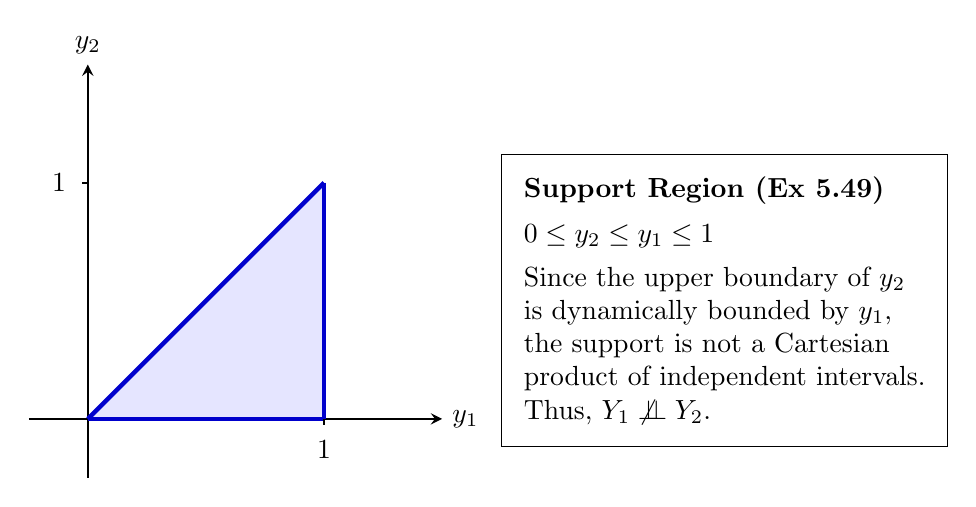
\begin{tikzpicture}[scale=1.5]
    % 1) Fill background
    \fill[blue!10] (0,0) -- (2,2) -- (2,0) -- cycle;
    
    % 2) Draw grid/axes
    \draw[thick, ->, >=stealth] (-0.5,0) -- (3,0) node[right] {$y_1$};
    \draw[thick, ->, >=stealth] (0,-0.5) -- (0,3) node[above] {$y_2$};
    
    % 3) Draw primary plots
    \draw[ultra thick, blue!80!black] (0,0) -- (2,2);
    \draw[ultra thick, blue!80!black] (2,2) -- (2,0);
    \draw[ultra thick, blue!80!black] (2,0) -- (0,0);
    
    % 4) Node labels
    \draw[thick] (2,0) -- (2,-0.05) node[below=2pt] {$1$};
    \draw[thick] (0,2) -- (-0.05,2) node[left=2pt] {$1$};
    
    % Single-node multiline legend
    \node[align=left, inner sep=8pt, anchor=west, draw, fill=white, text=black] at (3.5, 1) {
        \textbf{Support Region (Ex 5.49)} \\[4pt]
        $\displaystyle 0 \le y_2 \le y_1 \le 1$ \\[4pt]
        Since the upper boundary of $y_2$ \\
        is dynamically bounded by $y_1$, \\
        the support is not a Cartesian \\
        product of independent intervals. \\
        Thus, $Y_1 \not\indep Y_2$.
    };
\end{tikzpicture}
\end{center}

\subsection{Heuristics \& Pitfalls}
\begin{itemize}
    \item \textbf{Heuristic:} Before integrating to find marginals, look at the inequalities defining the support. If you see a variable bounding another variable (e.g., $y_1 < y_2$), immediately conclude they are dependent.
    \item \textbf{Pitfall (The Zero-Covariance Fallacy):} Assuming that if $\text{Cov}(Y_1, Y_2) = 0$, then $Y_1 \indep Y_2$. This is strictly false. Independence implies zero covariance, but zero covariance only implies lack of \textit{linear} dependence.
\end{itemize}

\newpage
\section{Part 5: Conceptual Synthesis and The "Big Picture"}

\subsection{A) Thematic Connections}
The central theme of this chapter is \textbf{using measure theory to formalize the absence of information flow}. In abstract algebra, we look for isomorphisms to show structures are identical; in probability, we look for product measures ($\mu_{1,2} = \mu_1 \times \mu_2$) to show structures are completely decoupled. This unifies previous topics in set theory (Cartesian products) and calculus (Fubini's Theorem for separable integrals).

\subsection{B) Forward and Backward Links}
\begin{itemize}
    \item \textbf{Backward Links:} This topic rigorously extends the basic discrete rule $\Prob(A \cap B) = \Prob(A)\Prob(B)$ into the continuous domain using Borel $\sigma$-algebras and Riemann/Lebesgue integration.
    \item \textbf{Forward Links:} Understanding independence is the absolute bedrock for \textbf{Stochastic Calculus} and \textbf{Martingale Theory}. For instance, Brownian Motion $W_t$ is defined by having \textit{independent increments} ($W_t - W_s \indep W_s$). Without the rigorous factorization theorems learned here, Ito's Lemma and the Black-Scholes equation cannot be derived.
\end{itemize}

\section{Part 6: Abstract Real-World Modeling (AI, ML, \& Quant Finance)}

\subsection{A) Concrete Scenarios}
\begin{enumerate}
    \item \textbf{Generative AI (Naive Bayes \& VAEs):} In Variational Autoencoders (VAEs), the latent space variables $\mathbf{z}$ are often forced to be independent standard normals, $p(\mathbf{z}) = \prod \mathcal{N}(z_i | 0, 1)$. The factorization theorem is used to compute the Kullback-Leibler divergence loss.
    \item \textbf{Quantitative Finance (Copulas \& CDOs):} In pricing Collateralized Debt Obligations (CDOs), quants must model the joint default probability of hundreds of assets. Assuming independence (factorization) drastically underestimates tail risk. The 2008 financial crisis was exacerbated by the misuse of the Gaussian Copula, which failed to capture extreme dependency during market crashes.
\end{enumerate}

\subsection{B) Model Problem Setup: Quantitative Finance Default Risk}
Let us build a rigorous model for two corporate bonds. Let $\tau_1, \tau_2$ be the random variables representing the time-to-default for Bond 1 and Bond 2.
\textbf{State Space:} $\Omega = \R_+ \times \R_+$.
\textbf{Marginal Measures:} Assume both follow an exponential distribution with hazard rate $\lambda$, so $F_i(t) = 1 - e^{-\lambda t}$.
\textbf{Optimization/Pricing Problem:} A derivative pays $\$1,000$ if \textit{both} bonds default before time $T=1$. 
If a junior quant falsely assumes independence, the price is proportional to:
\[ \Prob(\tau_1 \le 1, \tau_2 \le 1) = (1 - e^{-\lambda})^2 \]
However, using a rigorous \textbf{Clayton Copula} to model macroeconomic dependence (where $\theta > 0$ controls dependence):
\[ C(u, v) = (u^{-\theta} + v^{-\theta} - 1)^{-1/\theta} \]
The true joint probability is:
\[ \Prob(\tau_1 \le 1, \tau_2 \le 1) = \left( (1 - e^{-\lambda})^{-\theta} + (1 - e^{-\lambda})^{-\theta} - 1 \right)^{-1/\theta} \]
This model proves that as $\theta \to \infty$, the defaults become perfectly dependent, and the derivative price is vastly higher than the independent model suggests.

\newpage
\section{Part 7: Common Variations and Untested Concepts}

\subsection{Conditional Independence}
A critical concept missing from the basic homework is \textbf{Conditional Independence}, which is the foundation of Bayesian Networks and Markov Chains.
\begin{definition}
$X$ and $Y$ are conditionally independent given $Z$ (denoted $X \indep Y \mid Z$) if:
\[ f(x, y \mid z) = f(x \mid z)f(y \mid z) \]
\end{definition}

\textbf{Worked Example:} Let $Z \sim U(0,1)$. Given $Z=z$, let $X \sim \text{Exp}(z)$ and $Y \sim \text{Exp}(z)$ be independent. Are $X$ and $Y$ unconditionally independent?
\begin{proof}
The joint conditional density is $f(x, y \mid z) = z^2 e^{-z(x+y)}$.
To find the unconditional joint density, we integrate out $Z$:
\[ f(x, y) = \int_{0}^{1} z^2 e^{-z(x+y)} \, dz \]
This integral evaluates to a complex function of $(x+y)$ that \textit{cannot} be factored into $g(x)h(y)$. Thus, while $X \indep Y \mid Z$, they are \textbf{unconditionally dependent}. This proves that conditional independence does not imply marginal independence. $\blacksquare$
\end{proof}

\section{Part 8: Advanced Diagnostic Testing: "Find the Flaw"}

Below are five proofs containing a single, subtle logical or mathematical flaw. 

\textbf{Problem 1:} Let $X$ and $Y$ be random variables such that $\E[XY] = \E[X]\E[Y]$. \\
\textit{Proof of Independence:} Since the expectation of the product equals the product of the expectations, the covariance is zero. Therefore, the variables do not affect each other and $X \indep Y$. $\blacksquare$

\textbf{Problem 2:} Let $f(x,y) = 2e^{-(x+y)}$ for $0 \le x \le y < \infty$. \\
\textit{Proof of Independence:} We can factor the density as $f(x,y) = (2e^{-x})(e^{-y})$. Since the density factors into a function of $x$ and a function of $y$, by Theorem 5.5, $X \indep Y$. $\blacksquare$

\textbf{Problem 3:} Let $X_1, X_2, X_3$ be three coin tosses. We know $X_1 \indep X_2$, $X_2 \indep X_3$, and $X_1 \indep X_3$. \\
\textit{Proof of Mutual Independence:} Since every pair of variables is independent, the entire set of variables is mutually independent, meaning $\Prob(X_1, X_2, X_3) = \Prob(X_1)\Prob(X_2)\Prob(X_3)$. $\blacksquare$

\textbf{Problem 4:} Let $X, Y$ be continuous random variables. \\
\textit{Proof of Conditional Probability:} The probability that $X \in A$ given $Y = y$ is exactly $\Prob(X \in A \mid Y = y) = \frac{\Prob(X \in A \cap Y = y)}{\Prob(Y = y)}$. $\blacksquare$

\textbf{Problem 5:} Let $X, Y \sim \mathcal{N}(0,1)$ be independent. Let $U = X+Y$ and $V = X-Y$. \\
\textit{Proof of Independence:} $U$ and $V$ are linear combinations of independent normals. Since they are derived from independent variables, $U$ and $V$ must also be independent. $\blacksquare$

\vspace{2em}
\hrule
\vspace{1em}
\subsection*{Solution Key: Flaw Resolutions}
\textbf{Resolution 1:} \textit{Flaw:} Assuming zero covariance implies independence. \textit{Correction:} Zero covariance only implies lack of linear correlation. For example, if $X \sim U(-1,1)$ and $Y = X^2$, $\E[XY] = \E[X^3] = 0 = \E[X]\E[Y]$, but $Y$ is completely dependent on $X$.

\textbf{Resolution 2:} \textit{Flaw:} Ignoring the support constraint. \textit{Correction:} The support is $0 \le x \le y < \infty$, which is a triangle, not a Cartesian product. Theorem 5.5 strictly requires rectangular support. They are dependent.

\textbf{Resolution 3:} \textit{Flaw:} Conflating pairwise independence with mutual independence. \textit{Correction:} Pairwise independence does not guarantee mutual independence. (e.g., $X_1, X_2$ are independent coin flips, and $X_3 = X_1 \oplus X_2$. Any pair is independent, but the three together are completely dependent).

\textbf{Resolution 4:} \textit{Flaw:} Dividing by a zero-probability event. \textit{Correction:} For continuous variables, $\Prob(Y = y) = 0$. You cannot use discrete conditional probability formulas. You must use conditional density functions: $f(x|y) = f(x,y)/f_Y(y)$.

\textbf{Resolution 5:} \textit{Flaw:} Assuming any function of independent variables yields independent variables. \textit{Correction:} $U$ and $V$ are independent here \textit{only} because their covariance is $\text{Cov}(X+Y, X-Y) = \text{Var}(X) - \text{Var}(Y) = 1 - 1 = 0$, and they are jointly Gaussian. If $\text{Var}(X) \neq \text{Var}(Y)$, $U$ and $V$ would be dependent.

\end{document}